\subsubsection{{\bf RQ5. Analysis on Code Change Embeddings}}

To study the projections of the changed statements in the same and
different concerns, we first randomly chose the commits with two or
more clusters/concerns and in one of the cluster/concern, there are at
least two changed statements. Let us use $C$ to denote that
cluster/concern. We randomly chose two changed statements $S_1$ and
$S_2$ in $C$. We then randomly selected another changed statement
$S_3$ such that $S_3 \notin C$ and $S_3$ belongs to another cluster in
the same commit with $S_1$ and $S_2$. We measured the distance
$d_1(S_1,S_2)$ and $d_2(S_1,S_3)$. We repeated the process for all the
commits satisfying the above conditions until to get 384 triples of
($S_1, S_2, S_3$). Based on the population in our dataset, the size of
384 samples gives the confidence level of 95\% and the confidence
interval of 5\%.
%
We used statistical $p$-value to confirm our hypothesis
$H_1: d_1(S_1,S_2)$ $\leq$ $d_2(S_1,S_3)$. The null-hypothesis is
\textit{\textbf{$H_0: d_1(S_1,S_2) > d_2(S_1,S_3)$}}.

When we set the significance level $\alpha = 0.05$, the $p$-value is
$0.03$ (calculated on these 384 samples). In this case, the $p$-value
is smaller than $\alpha$, meaning the null hypothesis would be
rejected at the level of $\alpha = 0.05$. Therefore, our hypothesis
$H_1$: $d_1(S_1,S_2)$$ \leq$$ d_2(S_1,S_3)$ is confirmed.  That is,
the changed statements in the same concerns are projected nearer to
one another than the changed statements in different concerns. This
result is an indication that our {\em context-aware, graph-based
  embeddings for code changes are helpful for {\tool} in clustering the code
  changes via the embeddings into different concerns}.


%\textit{\textbf{$H_1: d_1(S_1,S_2) \leq d_2(S_1,S_3)$}}

%Moreover, we also reported the examples where the same changed
%statements in different concerns are projected farther away in the
%vector space.


%To better understand the quality of the code change embeddings, in this RQ, we selected 384 triples of ($S_1, S_2, S_3$) as the statistical analysis sample based on the confidence level of $95\%$ and the confidence interval $5\%$. Our hypothesis for the quality of code change embedding is that $d_1(S_1,S_2)$ $\leq$ $d_2(S_1,S_3)$.

% which means that our code change embeddings are in good quality.

%\begin{figure}[t]
%	\centering
%	\lstset{
%		numbers=left,
%		numberstyle= \tiny,
%		keywordstyle= \color{blue!70},
%		commentstyle= \color{red!50!green!50!blue!50},
%		frame=shadowbox,
%		rulesepcolor= \color{red!20!green!20!blue!20} ,
%		xleftmargin=1.5em,xrightmargin=0em, aboveskip=1em,
%		framexleftmargin=1.5em,
%		numbersep= 5pt,
%		language=Java,
%		basicstyle=\scriptsize\ttfamily,
%		numberstyle=\scriptsize\ttfamily,
%		emphstyle=\bfseries,
%		moredelim=**[is][\color{red}]{@}{@},
%		escapeinside= {(*@}{@*)}
%	}
%	\begin{lstlisting}[]
%//-----------------------------------Concern-1-------------------------------
%    private void Dispose(bool disposing)
%    {
%(*@{\color{red}{-     \space \space\space\space\space\space\space\space      if% (this.disposed)}@*)
%(*@{\color{cyan}{+    \space\space\space\space\space\space\space\space\space   %     if (disposed)}@*)
%        {
%            return;
%        }
%        ...
%    }
%
%//-----------------------------------Concern-2-------------------------------
%    private HelpText AddOption(string requiredWord, int maxLength, OptionSpecification option, int widthOfHelpText)
%    {
%        ...
%        if (option.ShortName.Length > 0)
%        {
%(*@{\color{red}{-\space\space\space\space\space\space\space\space\space\space  %      if (this.addDashesToOption)}@*)
%(*@{\color{cyan}{+\space\space\space\space\space\space\space\space\space\space %      if (addDashesToOption)}@*)
%	    	{
%			    optionName.Append('-');
%	    	}
%    	...
%    }
%
%    internal HelpText AddToHelpText(HelpText helpText, bool before)
%    {
%        return before
%(*@{\color{red}{- \space\space\space\space\space\space\space\space               ? this.AddToHelpText(helpText, line => helpText.AddPreOptionsLine(line)) : this.AddToHelpText(helpText, line => helpText.AddPostOptionsLine(line));}@*)
%(*@{\color{cyan}{+  \space\space\space\space\space\space\space\space 	? AddToHelpText(helpText, helpText.AddPreOptionsLine) : AddToHelpText(helpText, helpText.AddPostOptionsLine);}@*)
%    }
%	\end{lstlisting}
%	\vspace{-15pt}
%	\caption{Example for RQ5}
%	\vspace{-6pt}
%	\label{RQ5-example}
%\end{figure}
			
%The code in Figure \ref{RQ5-example} shows an example that contains two concerns. The statement in $Line-4$ in concern-1 is very similar to the statement in $Line-18$ in concern-2. Following the statistical analysis procedure, we pick the statement in $Line-4$ as $S_3$, the statement in $Line-18$ as $S_2$, and the statement in $Line-29$ as $S_1$. Then we calculate the $d_1(S_1,S_2)$ and $d_2(S_1,S_3)$ by using \tool to generate the representation vectors for each changed statement. The results are $d_1(S_1,S_2) = 0.285$ and $d_2(S_1,S_3)=0.491$. This result proves that the similar changed statements in different concerns are projected farther away in the vector space when \tool generates the embedding vectors for the code change statements. It also shows that \tool learns the context information well to distinguish the differences between the similar code changes in a different context.

\begin{figure}[t]
	\centering
	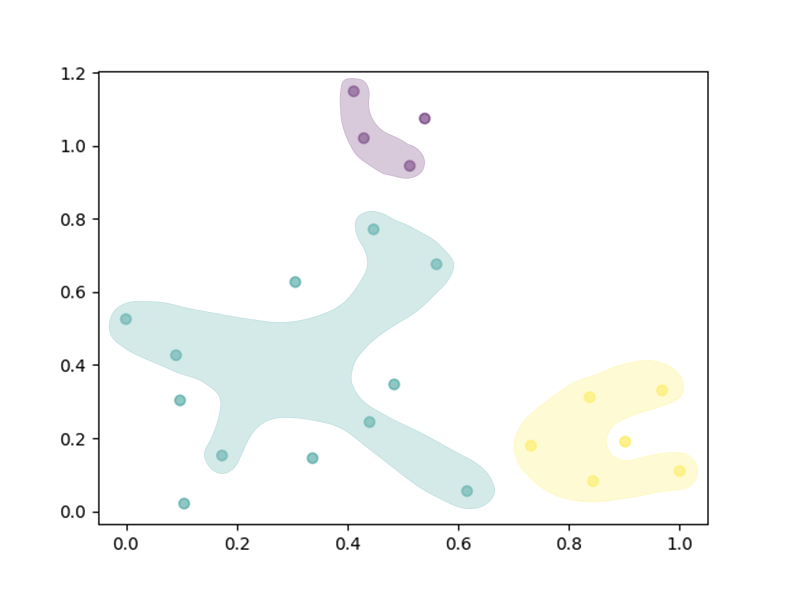
\includegraphics[width=2.1in]{figures/RQ5.png}
	\vspace{-18pt}
	\caption{Code Change Embedding Visualization via t-SNE}
	\label{fig:vis}
\end{figure}

For illustration, we randomly picked a commit in our above
sample. The commit contains three concerns in which one concern has 4
changed statements, another one has 12 changed statements, and the
last one has 6 changed statements. We used the $t$-distributed
stochastic neighbor embedding (t-SNE)~\cite{tsne} to visualize the
embeddings of the changed statements in the vector space. t-SNE is a
statistical method for visualizing high-dimensional data by giving
each data point its projected location in a two-dimensional vector
space. As seen in Figure~\ref{fig:vis}, we marked the embeddings for
the changed statements in each concern with a different color. The
correctly clustered changes are within the corresponding boundary for
a concern. Despite that {\tool} misclassified a few statements,
we can observe that the changes in each concern are projected to the
nearby locations in the vector space. This figure illustrates that the
our code change embeddings facilitate our supervised-learning
clustering model to correctly cluster the changed statements.




%To better understand the code change embedding quality, we randomly pick one commit that contains three concerns. And for each concern among them, it contains 4, 12, and 6 statements, respectively. By using the t-SNE model \cite{} in scikit-learn \cite{} package, we can have the visualization results shown in Figure~\ref{fig:vis}. From Figure~\ref{fig:vis}, we can see that the statements in three concerns are in different colors(Purple for concern 1, cyan for concern 2, and yellow for concern 3), and the statements that are correctly clustered by \tool are inside of the same color boundary. From the colored nodes and boundaries, we can see that the same colored statements are gathered into groups. It proves our hypothesis that the changed statements in the same concerns are projected nearer to one another than those in different concerns from the visualization direction.
